\documentclass[main.tex]{subfiles}
\usetikzlibrary{decorations.pathmorphing,patterns}
%% Current Author: SEQ
\setcounter{chapter}{10}
\begin{document}
\chapter{Oscillations}
\section{Simple Harmonic Motion}
\spec{Recall the condition for simple harmonic motion and hence identify situations in which simple harmonic motion will occur}


Any oscillation where the acceleration is proportional to the displacement from an equilibrium position and in the opposite direction to the displacement is described as Simple Harmonic Motion (SHM).

These two conditions can be expressed in equation form as:
\[ a \propto -x \]
Notice the minus sign to signify that the acceleration is in the opposite direction to the displacement.

We will mainly be looking at idealised springs and pendulums to understand the maths behind it but the real reason for studying SHM is that it is an excellent approximation for many of the oscillations that we come across in the natural world.

So while the topic is introduced with some rather prosaic examples this provides the building blocks to understanding earthquakes or how atoms vibrate in lattices as well as any musical instrument you can think of.

%\pagebreak

So without further ado let's look at our first and perhaps simplest example.

A mass on a spring on a smooth horizontal surface.
\vspace{0.2in}


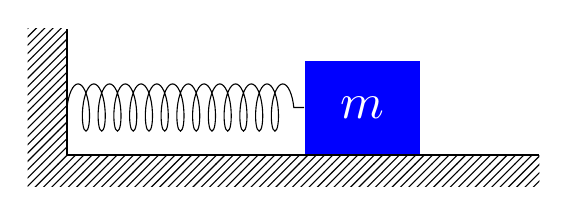
\begin{tikzpicture}
\node[rectangle,scale = 1.8, fill=blue,inner sep=2.5mm, text = white] (a) at (3.75,3) {$m$};


\draw[decoration={aspect=0.3, segment length=2mm, amplitude=3mm,coil},decorate] (0,3) -- (a); 

\fill [pattern = north east lines] (0,2) rectangle (6,2.4);
\fill [pattern = north east lines] (-.5,2) rectangle (0,4);
\draw[thick] (0,2.4) -- (6,2.4);
\draw[thick] (0,2.4) -- (0,4);

\end{tikzpicture}

What happens if we move the mass by a distance x and then let it go?

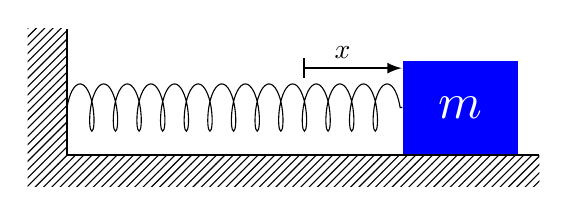
\begin{tikzpicture}
\node[rectangle,scale = 1.8, fill=blue,inner sep=2.5mm, text = white] (a) at (5,3) {$m$};




\draw[decoration={aspect=0.3, segment length=3mm, amplitude=3mm,coil},decorate] (0,3) -- (a); 

\fill [pattern = north east lines] (0,2) rectangle (6,2.4);
\fill [pattern = north east lines] (-.5,2) rectangle (0,4);
\draw[thick] (0,2.4) -- (6,2.4);
\draw[thick] (0,2.4) -- (0,4);
\draw[thick, |-latex] (3,3.5) -- (4.25,3.5);
\node at (3.5,3.7) {$x$};
\end{tikzpicture}


Before going into any mathematical detail we can think about what will happen to the mass.
\begin{itemize}
\item We know that there is now a force from the stretched string which is pulling the mass back to its original position. 
\item This will cause the mass to accelerate to the left. 
\item Once the mass reaches its starting point it will overshoot and start compressing the spring.
\item This creates a resultant force which will again restore the mass to its original position.
\item This will cause the mass to accelerate to the right.
\item The mass will overshoot again and the cycle will continue.
\end{itemize}
Note that the direction of the acceleration is always opposite to the displacement.

The mathematical treatment for this starts very simply with a basic knowledge of Hooke's law.

The force on a stretched or compressed spring is given by 
\[
F=-kx
\]
where k is the spring constant.

Newton's second law tells us that 
\[
F=ma
\]

Putting these together we get
\[
a = \dfrac{F}{m}=-\dfrac{k}{m}x
\]
Because k and m are constant this satisfies the condition for SHM,
\[
a \propto -x
\]

\begin{example}
A  2kg mass attached to a horizontal spring of spring constant 0.3Nm$^{-1}$ is stretched by 10cm and then released.

Find the maximum acceleration of the mass


	\vspace{1cm}

		

		\textbf{Answer}

Using the formula $a = -\dfrac{k}{m}x$
The maximum acceleration will occur when x is a maximum so 
\[
acceleration_{max} = - \dfrac{0.3}{2} \times 0.1
\]
\[
acceleration_{max} = -0.015 ms^{-2}
\]

\end{example}






\spec{* show that the condition for simple harmonic motion leads to a differential equation of the form
\[ 
\dfrac{d^2x}{dt^2} = - \omega^2 x
\]
and that 
\[ 
x = A cos \omega t 
\] 
is a solution to this equation}


Acceleration is the rate of change of velocity 

\[
a = \dfrac{dv}{dt} 
\]

and velocity is the rate of change of displacement

\[
v = \dfrac{dx}{dt} 
\]

Putting these two together gives the condition for simple harmonic motion as.

\[
\dfrac{d^2x}{dt^2}=-\omega ^2 x
\]

where $\omega ^2$ is a (strange choice) of constant.

This is a second order differential equation and to solve it we need to find a function which when differentiated twice gives us the negative of the original function.

By inspection we can see that functions with $\sin \omega t$ and $\cos \omega t$ are both possible solutions.

e.g.

\begin{align*} 
x &= A cos \omega t \\
\dfrac{dx}{dt} &= - A\omega sin \omega t \\
\dfrac{d^2x}{dt^2} &= -A\omega^2 cos \omega t = -\omega ^2 x \\
\end{align*}

So $x= Acos \omega t$ is a solution (using sin is equivalent but with a phase offset.)

Looking at this function we can see that it will give us a cosine wave with an Amplitude of A and a time period of $ \dfrac{2 \pi}{\omega}$.

This gives us a frequency on $\dfrac{1}{T} = \dfrac{\omega}{2 \pi}$

So $\omega$ is the angular frequency (which explains our strange choice of constant).

\begin{tikzpicture}
	%curve
		\draw (0.5,1) cos (1.5,0) sin (2.5,-1) cos (3.5,0) sin (4.5,1) cos
			(5.5,0) sin (6.5,-1) cos (7.5,0) sin (8.5,1) cos (9.5,0)
			sin (10.5,-1) cos (11.5,0);
	% zero crossing
		\draw[dotted] (0.5,0) -- (11.5,0);
	%axis + labels
		\draw [<->] (0.5,1) -- (0.5,-1);
		\draw [->] (0.5,0) -- (11.5,0);
		\node at (11.7,0) {$t$};
		\node at (0.5,1.2) {$+A$};
		\node at (0.5,-1.2) {$-A$};
		\node at (0.3,0) {$0$};
	%Time period description
		\draw [<->] (4.5,1.15) -- (8.5,1.15);
		\node at (6.5,1.6) {Time period, $\dfrac{2 \pi}{\omega}$};
	%Amplitude description
		\draw [<->] (6.5,0) -- (6.5,-1);
		%to stop line overlap
		\draw [fill=white,ultra thick,white] (7,-0.3) rectangle (9,-0.7); 
		\node at (8, -0.5) {Amplitude, $A$};
\end{tikzpicture}

We now have a general expression for the displacement x of the object after a time t.

The value of $\omega$ will be given by the physical properties of the system.

e.g.
For the mass on a spring we looked at earlier

\begin{align*} 
F &= -kx && \text {Force on mass by Hooke's Law}\\
a &= -\dfrac{k}{m} x  && \text{gives acceleration}\\
\dfrac{d^2x}{dt^2} &= -\omega ^2 x && \text{comparing with condition for SHM} \\
\omega ^2 &= \dfrac{k}{m} && \text{gives value for constant } \omega \\
\omega &= \sqrt{\dfrac{k}{m}} \\
\end{align*}

\spec{* use differential calculus to derive the expressions
\[
v=-A \omega sin \omega t 
\] and 
\[a = -A\omega^2 cos \omega t 
\] 
for simple harmonic motion.}



This is very simply achieved by differentiating our expression for displacement with respect to time as velocity =$\dfrac{dx}{dt}$ and acceleration = $\dfrac{dv}{dt}$

Remember that the differential of cos is -sin.

so 
\[
x = A cos \omega t
\]
\[
v = \dfrac{dx}{dt}= -A \omega sin \omega t
\]
\[
a = \dfrac{dv}{dt}= -A \omega^2 cos \omega t
\]

\spec{ understand the phase differences between displacement, velocity and acceleration in simple harmonic
motion}

Plotting these equations onto a graph gives the following.




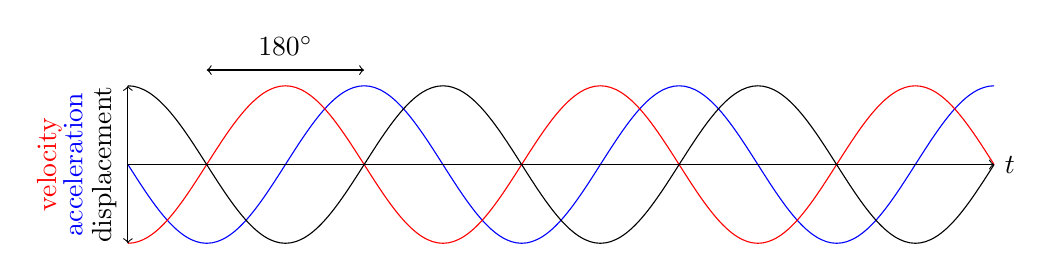
\begin{tikzpicture}
	%curve 1
		\draw[blue] (0.5,0) sin (1.5,-1) cos (2.5,0) sin (3.5,1) cos (4.5,0) 
			sin (5.5,-1) cos (6.5,0) sin (7.5,1) cos (8.5,0) sin (9.5,-1) 
			cos (10.5,0) sin (11.5,1);
	%curve 2
    \draw[red] (0.5,-1) cos (1.5,0) sin (2.5,1) cos (3.5,0) sin (4.5,-1) cos
			(5.5,0) sin (6.5,1) cos (7.5,0) sin (8.5,-1) cos (9.5,0)
			sin (10.5,1) cos (11.5,0);
		cos (10.5,0) sin (11.5,1);
    %curve 3
        	\draw (0.5,1) cos (1.5,0) sin (2.5,-1) cos (3.5,0) sin (4.5,1) cos
			(5.5,0) sin (6.5,-1) cos (7.5,0) sin (8.5,1) cos (9.5,0)
			sin (10.5,-1) cos (11.5,0);
	% zero crossing
		\draw[dotted] (0.5,0) -- (11.5,0);
	%axis + labels
		\draw [<->] (0.5,1) -- (0.5,-1);
		\draw [->] (0.5,0) -- (11.5,0);
		\node at (11.7,0) {$t$};
		\node[rotate=90] at (0.2,0) {displacement};
        \node[rotate=90, blue] at (-0.2,0) {acceleration};
        \node[rotate=90, red] at (-0.5,0) {velocity};
	%Phase difference description
		\draw [<->] (1.5,1.2) -- (3.5,1.2);
		\node at (2.5,1.5) {$180^\circ$};
\end{tikzpicture}



Note the phase shift between displacement, velocity and acceleration.

Velocity is $\dfrac{\pi}{2}$ or $90^\circ$out of phase with displacement.

Acceleration is $\pi$ or $180^\circ$ out of phase with displacement.

So when acceleration or displacement has a maximum magnitude, the velocity is zero


\spec{ *recognise and use the expressions $x = A cos\omega t, v = -A \omega sin \omega t, a = -A \omega^2 cos \omega t$ and $F = –m \omega^2x$ to solve problems}

We can use these equations to solve problems by identifying the variables and substituting.

The last equation is a combination of $a = -\omega^2 x$ and $F = ma$

\begin{example}


A mass attached to a spring is set into motion on a horizontal frictionless surface. The amplitude of oscillation is 15mm and it takes 5 seconds to perform 20 oscillations.

Calculate the time period and frequency.

Hence calculate the velocity and acceleration after 9.3 seconds.

	\vspace{1cm}
    
\textbf{Answer}

The first part doesn't require any knowledge of SHM. If there are 20 oscillations in 5 seconds this means $\dfrac{20}{5}$ oscillations in one second.

So $f=4Hz$

and $T = \dfrac{1}{f} = 0.25s$

Now that we have the frequency we can calculate the angular frequency $\omega = 2 \pi f = 8 \pi$

We are given the amplitude A as 15mm and the time is 9.3 seconds so we can now use our SHM formulae.

So for the velocity

\[
v=-A \omega sin \omega t 
\]

\[
v = -15 \times 8 \pi sin (8 \times \pi \times 9.3)
\]
\[
v = -360 mms^{-1} = .36ms^{-1}
\]

and for acceleration

\[
a = \dfrac{dv}{dt}= -A \omega^2 cos \omega t
\]

\[
a = 15 (8 \times \pi)^2 cos (8 \times \pi \times 9.3)
\]

\[
a = 2900 mms^{-2} = 2.9ms^{-2}
\]


\end{example}



\spec{ recall and use $T = \dfrac{2 \pi}{\omega}$
as applied to a simple harmonic oscillator}



\spec{ *show that the total energy of an undamped simple harmonic system is given by $E = \dfrac{1}{2}mA^2\omega^2$ and
recognise that this is a constant}

\spec{ recognise and use $E = \dfrac{1}{2}mA^2\omega^2$ to solve problems}
\spec{ distinguish between free, damped and forced oscillations}
\spec{ recall how the amplitude of a forced oscillation changes at and around the natural frequency of a system
and describe, qualitatively, how damping affects resonance.}

\end{document}

%sagemathcloud={"latex_command":"latexmk -pdf -f -g -bibtex -synctex=1 -interaction=nonstopmode '11-oscillations.tex'"}
